\section{Implementation}
Our VizAPI tool includes two main phases: (1) data extraction and (2) visualization. The data extraction
phase uses static and dynamic analysis to collect data about client usages of libraries. The visualization
phase transforms the data into d3 format and makes it available to users.

\subsection{Static Analysis}
\label{sec:static}

We use Javassist~\cite{chiba00:_load_struc_reflec_java} to perform
class hierarchy analysis on clients and create a static call graph. We
collect data about client usages of libraries by running client test
suites under instrumentation. The instrumentation records API uses
which cross client/library boundaries, closely mirroring the API usage
patterns that we describe in Section~\ref{sec:patterns}.  At the same
time, we also use Javassist to instrument the code so that we can
collect dynamic analysis data.   \\

\begin{figure*}[h]
 \begin{center}
\resizebox{0.9\textwidth}{!}{
  \begin{tikzpicture}
    \node[block] (client) {client};
    \node[block,below=1cm of client] (library) {library};

    \draw (library) -- node[left] (depends) {depends on} (client);

    \node[above left=.75em of client] (ja) {\begin{minipage}{7em} modify \\with Javassist \end{minipage}};
    \draw[-Latex] (ja) -> (client);
    \draw[-Latex] (ja) to [->,bend right=35] (library.west);

    \node[block, above right=2em of client,xshift=-2em] (olib) {other library};
    \draw (client) -- node[right,xshift=.1em] (also) {also depends on} (olib);

    \node[oval,right=of depends] (test) {maven: run tests};

    \draw[-Latex] (client) to [->,bend left=15] (test);

    \node[block, right=10em of client] (output) {test output};
    \node[block, right=10em of library] (raw) {raw API usage info};

    \draw[-Latex] (test) to (output);
    \draw[-Latex] (test) to (raw);

    \node[oval, right=of raw] (Py) {Python scripts};
    \draw[-Latex] (raw) to (Py);

    \node[block, right=1em of Py] (viz) {D3 visualizations};
    \draw[-Latex] (Py) to (viz);
  \end{tikzpicture}
}
  \caption{Our instrumentation workflow. Using Javassist, we analyze and instrument clients and run their test suites. (We process the generated data with Python scripts to create D3 visualizations for VizAPI.)}
  \label{fig:workflow}
 \end{center}
\end{figure*}

Figure~\ref{fig:workflow} summarizes our instrumentation and
data capture workflow. We next describe our instrumentation implementation in detail.

We identify interactions across the client/library boundaries by inspecting JAR files of
each software component to obtain a list of classes for every component. We associate classes 
and their members to components based on these lists. Since the JAR files contain source code,
we ensure that none of the library uses meant solely for unit testing are captured.

\paragraph{Vanilla invocations}
The standard case is simple. At every invoke instruction in every
loaded method which transfers control between the client and the
library, we add code to record that invoke by incrementing a counter.
We handle both static and virtual (including special, virtual,
interface, and dynamic) calls. Crossing the client/library boundary
includes conventional calls from the client to the library as well as callbacks from the library to the client.  

\paragraph{Field accesses}
We capture direct (field sets and gets) and reflective (via invocations of
\texttt{java.lang.reflect.Field.get()} and \texttt{.set()}) field
accesses.

\paragraph{Dynamic proxies and reflective calls}
We specially handle invocations of the distinguished method 
\texttt{java.lang.reflect.Method.invoke()} method used to invoke dynamic proxies and reflective calls, recording
details of the calls that we intercept. 
We identify dynamic proxies by checking whether the invocation 
of \texttt{Method.invoke()} originates from a class that implements 
\texttt{java.lang.reflect.InvocationHandler}. If so,
we inspect the call stack to find the caller and callee of 
\texttt{Method.invoke()} and record the call if it crosses the client/library boundary. 
All other calls to \texttt{Method.invoke()} are standard reflective calls, 
and we record the respective callers and callees.
(We also specifically ignore calls to \texttt{Method.invoke()} made by the Maven surefire plugin
as it runs tests.)
% \todo[inline]{When running tests, the Maven surefire plugin uses the invoke method too,
% which is ignored. Should we talk about that?}

Instrumenting methods also allows us to capture several other library uses,
as we describe below.

\paragraph{Class usages}
We capture reflective uses of the \texttt{Class} object by intercepting calls to
\texttt{java.lang.Class.forName()} and \texttt{java.lang.ClassLoader.loadClass()}.

\paragraph{Service Loaders} We are particularly interested in bypasses of 
services that use the \texttt{ServiceLoader} API. Before the instrumentation, we record a list 
of services and their implementations by inspecting files in \texttt{src/main/resources/META-INF/services}.
With this information, we look for service bypasses which are direct uses of service implementation 
classes in clients, either through instantiations, casts or reflection. We also intercept calls 
to method \texttt{load()} in classes with name \texttt{Service*Loader} and record any calls to methods beyond 
the published interface.

\paragraph{setAccessible()} 
Java provides the \texttt{setAccessible()} method to allow reflective access to class members despite
access modifiers. After a call to this method, the program may then (subject to security manager restrictions)
reflectively access the class member.
We thus record calls to \texttt{setAccessible()} along with the previous visibility of the class member.

\paragraph{Annotations} 
We have a quasi-static approach for finding class, field and method
annotations: we observe all annotations for a class or class member
when it is loaded, and record cases where a class or member declares an
annotation from the library of interest. We also record an association
between the class and its memers' annotations.

\paragraph{Inheritance and interface implementation} At load time,
we also record information about all superclasses and implemented interfaces
that cross the library/client barrier.

\paragraph{Instantiations and casts} We also instrument the
\texttt{NewExpr} and \texttt{Cast} bytecodes to record library/client 
instantiations and casts.

\subsection{Dynamic Analysis}
We modify the build system of each
client (Maven) to run its provided tests on instrumented
code, obtaining dynamic call graphs.

\todo{more details on the dynamic call graphs}

We executed each of the clients' test suites to collect data about how the clients use all of their dependencies; our data therefore includes not just interactions between our clients and the 11 libraries sampled, but also ``bycatch''---that is, other libraries that are also called by the clients (``also depends on'' in Figure~\ref{fig:workflow}) and the libraries. The total static transitive closure of dependencies of our clients includes 4297 components.

Collecting execution data from programs is more challenging than it seems: downloading software and collecting static numbers is fairly straightforward, but running this software to instrument it involves fixing numerous uninteresting environment glitches which nevertheless block progress---even in the stable environment of a continuous integration system at a large software company, Kerzazi et al~\cite{kerzazi14:_why_do_autom_build_break} found that 17.9\% of builds break, and our context is even more challenging.

While our current benchmark set consists of 101 projects, it is possible to run both our static and dynamic analysis tool and the VizAPI visualization tool on new libraries and clients. However, when either tool is run by a library developer, they are required to provide a specific set of clients that they wish to observe as input to the tools. Libraries.io can be used to find popular clients of libraries---it provides a dependency tree based on projects' packaging information.


\subsection{Visualization System}
\label{subsec:vis-system}

\begin{figure*}[h]
\begin{center}

\subfloat[Usage Scenario 1: Library \textit{jsoup} (pink with dark borders), called by two clients, \textit{ez-vcard} (hollow with purple border) and \textit{JsoupXpath} (hollow with pink border). Exploration shows that internal jsoup packages aren't called directly by clients.
\label{fig:usagescenario1}]
{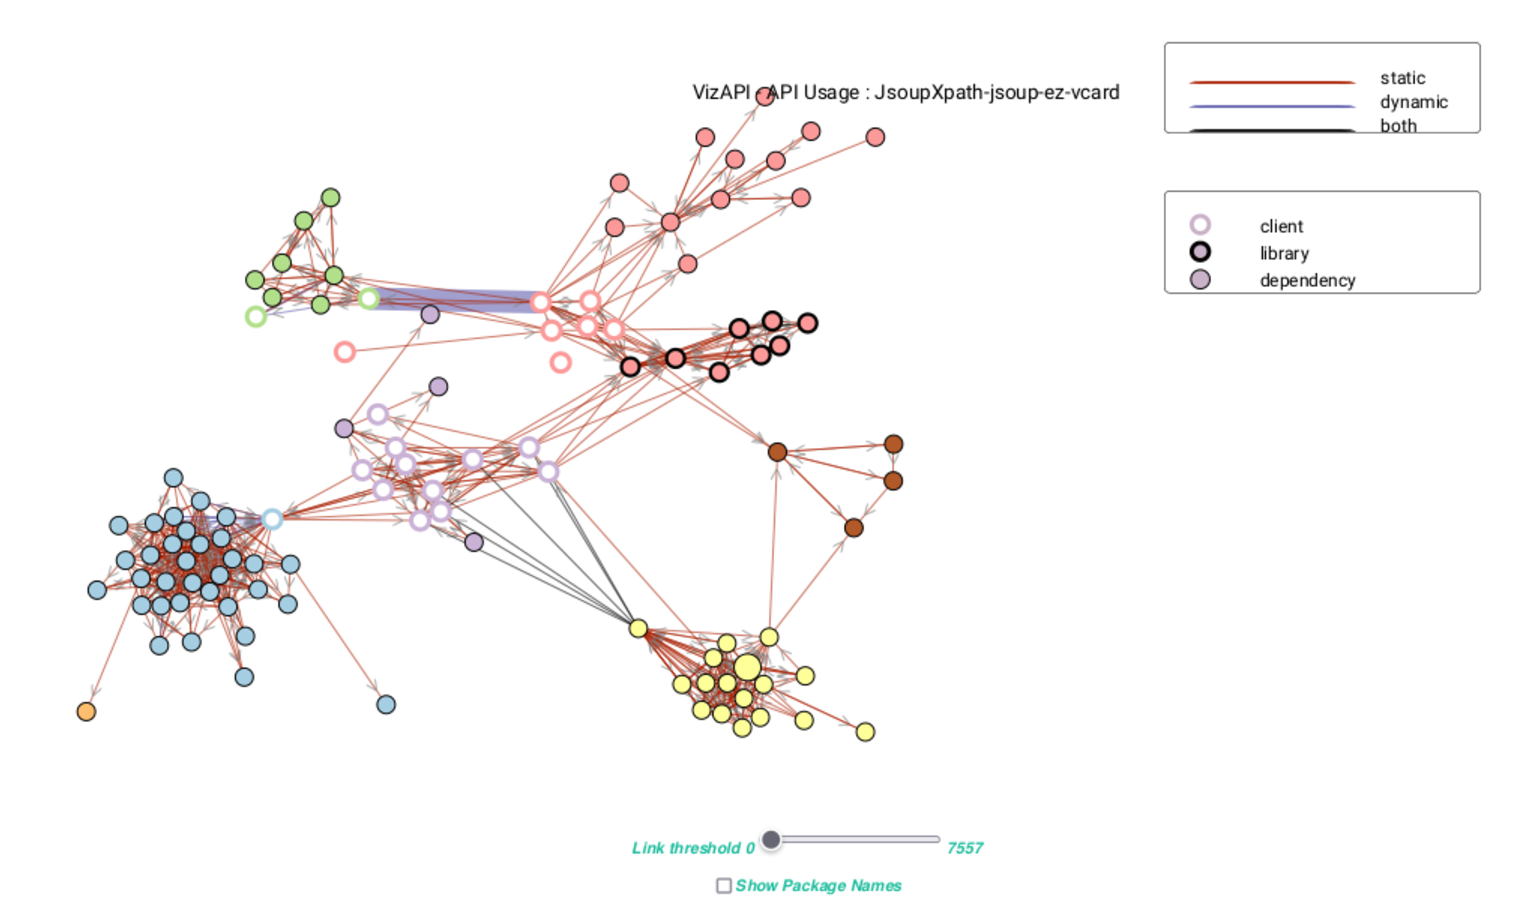
\includegraphics[width=16cm]{images/usage-scenario1.pdf}}
\hspace{7mm}

\subfloat[Usage Scenario 2: Client \textit{dataprocessor} (hollow, orange border) calls only one package in library \textit{fastjson} (green fill).
\label{fig:usagescenario2}]
{
\makebox[16cm]{
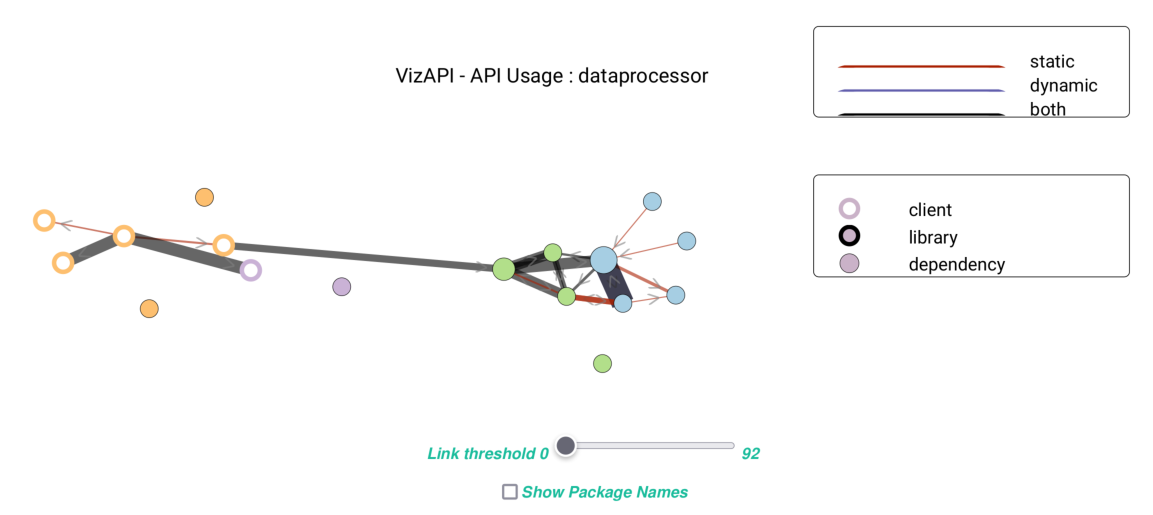
\includegraphics[width=11cm]{images/usage-scenario2.pdf}
}
}
\caption{\label{fig:usagescenarios} VizAPI Usage Scenarios.}

\end{center}
\end{figure*}


Once we have generated data from our tool that runs the static and dynamic analyses, we use a modified version
of the d3graph\footnote{\url{https://pypi.org/project/d3graph/}} library in Python to generate a d3js\footnote{\url{https://d3js.org/}}
visualization. The modifications that we made to the d3graph  library in Python in Python include multiple styling changes (for example, changing node styles based on whether it is a client, library or dependency),
legends and a toggle to show all package names. 
The graphs in Figures~\ref{fig:example}, \ref{fig:usagescenario1} and \ref{fig:usagescenario2} are examples of graphs produced by VizAPI.

VizAPI graphs are force-directed graphs based on the frequency of
interactions between different software components.  Each node is a
set of one or more packages that belong to the same JAR.  There are
three categories of nodes: clients are represented by nodes with white
interiors; libraries by nodes with filled interiors and black borders;
and dependencies (called by libraries but not clients) by nodes with
filled interiors and normal borders.  We coalesce nodes if they
originate from the same JAR and have the same incoming and
outgoing edges.

Each edge is directed
from the source package(s) to the target package(s) and represents an interaction 
(invocations, fields, annotations, subtyping) between packages. 
The thickness of each edge reflects the frequency of interactions between the source and the target.
Double-clicking on a node emphasizes its direct interactions with other packages while fading out the rest of the graph.

We run a Python implementation of the Louvain clustering algorithm~\cite{blondel2008fast}, and make the clusters 
visible by colouring nodes based on cluster.
This means that the same colour could indicate nodes (of the same category) from the same or different JARs.
Hovering on a node shows the list of packages and 
the JAR that they belong to, 
formatted as “jar : $\langle$space separated list of packages$\rangle$”. 
